\documentclass[portrait,a1,final]{a0poster} % a0poster class sets the paper size
\usepackage[utf8]{inputenc}
\usepackage[english]{babel}
\usepackage[pdftex]{graphicx}
\usepackage[ELEC,RGB]{aaltologo} % RGB, Coated, Uncoated
\usepackage{lipsum} % Lorem ipsum generator
\usepackage{titlesec} % For changing the font on chapters, sections, etc.
\usepackage{caption}
\usepackage{wrapfig}

\usepackage{titlesec}
\titleformat*{\subsection}{\normalsize\bfseries}

%% Section font size reduction for a1 posters %%%%%%%%%%%%%%%%%%%%%%%%%%%%%%%%%%%%%%%%%

% Also changes the format to sans serif bold, i.e. bold Helvetica via aaltologo package, can change the color of section text

\titleformat{\section}{\large\bfseries\sffamily\color{aaltoPurple}}{\textcolor{aaltoPurple}{\thesection}}{1em}{} % Text size for a1 posters

%\titleformat{\section}{\large\bfseries\sffamily\color{aaltoBlack}}{\textcolor{aaltoBlack}{\thesection}}{1em}{} % Text size for a1 posters

%\titleformat{\section}{\large\bfseries\sffamily}{\thesection.}{1em}{} % Text size for a1 posters with a dot after the incremental number

%%%%%%%%%%%%%%%%%%%%%%%%%%%%%%%%%%%%%%%%%%%%%%%%%%%%%%%%%%%%%%%%%%%%%%%%%%%%%%%%%%%%%%%


\usepackage{epstopdf} % so that ``pdflatex'' accepts .eps files


% Safe alternative math font for aaltoseries (optional)
\usepackage{fouriernc}


% Teach hyphenation for alien words
\hyphenation{op-tical net-works semi-conduc-tor}






%\newcommand{\vt}[1]{\ensuremath{\boldsymbol{#1}}} % vector, i.e. math bold face, cursive
\newcommand{\vt}[1]{\ensuremath{\mathbf{#1}}} % vector, i.e. math bold face, not-cursive
\newcommand{\lt}[1]{\ensuremath{\mathrm{#1}}} % sub or sup text, i.e. not cursive
\newcommand{\ec}{\ensuremath{\vt{J}}} % electric surface current
\newcommand{\mc}{\ensuremath{\vt{M}}} % magnetic surface current
%
\newcommand{\aee}{\ensuremath{\overline{\overline{a}}_\lt{ee}}}
\newcommand{\aem}{\ensuremath{\overline{\overline{a}}_\lt{em}}}
\newcommand{\ame}{\ensuremath{\overline{\overline{a}}_\lt{me}}}
\newcommand{\amm}{\ensuremath{\overline{\overline{a}}_\lt{mm}}}
\newcommand{\bee}{\ensuremath{\overline{\overline{b}}_\lt{ee}}}
\newcommand{\bem}{\ensuremath{\overline{\overline{b}}_\lt{em}}}
\newcommand{\bme}{\ensuremath{\overline{\overline{b}}_\lt{me}}}
\newcommand{\bmm}{\ensuremath{\overline{\overline{b}}_\lt{mm}}}
%
\newcommand{\adyad}{\ensuremath{\overline{\overline{a}}}}
\newcommand{\bdyad}{\ensuremath{\overline{\overline{b}}}}
%
\newcommand{\unitx}{\ensuremath{\vt{x}_0}}
\newcommand{\unity}{\ensuremath{\vt{y}_0}}






\newcommand{\sectionspace}{10mm} % Free space before each section inside a minipage
\newcommand{\figurespace}{10mm} % Free space around figures inside a minipage (where floats are not allowed)


\begin{document}


\thispagestyle{empty} % Removes the page number


\begin{minipage}[t]{1\linewidth} % The first minipage for the logo & title
\vspace{0pt} % A trick to align the parallel minipages on top

\vspace{0.008\linewidth} % Increase the top margin

\begin{minipage}[t]{0.28\linewidth} % logo
\vspace{0pt} % Alingns the parallel minipages on top

%% Choose the logo or use random generator
\AaltoLogoLarge{1.55}{''}{aaltoYellow} % Chosen logo, scaled for A1 size
%\AaltoLogoRandomLarge{1.55} % Random logo, scaled for A1 size

\end{minipage} % no empty line before the next begin
\begin{minipage}[t]{0.7\linewidth} % title
\vspace{0pt} % Alingns the parallel minipages on top


%% Font sizes for a0poster are
%\tiny
%\scriptsize
%\footnotesize
%\small
%\normalsize
%\large
%\Large
%\LARGE
%\huge
%\Huge
%\veryHuge
%\VeryHuge
%\VERYHuge

%% Official colors from aaltologo-package (visual-identity guideline)
% aaltoBlack
% aaltoGray
% aaltoGrayScale (for b&w prints)
% aaltoYellow
% aaltoOrange
% aaltoRed
% aaltoFuchsia
% aaltoPurple
% aaltoBlue
% aaltoTurquoise
% aaltoGreen
% aaltoLightGreen
% You can use \textcolor{<aaltocolor>}{<your text>) to change the colors of text, or

% Aalto-fancy title, use \baselinestretch to change linespacing, \textit{} for italic text, \textcolor for colored text
{\renewcommand{\baselinestretch}{0.6} % Changes the baseline skip smaller for the title
\textcolor{aaltoGreen}{\Huge{\bfseries{\textsf{Techniques and tools for measuring \\energy efficiency of scientific software applications}}}} % Text size for a1 posters
\par} % <- for \baselinestretch

%% More conservative title, upright and black
%{\renewcommand{\baselinestretch}{0.85} % Changes the baseline skip smaller for the title
%\Huge{\bfseries{\textsf{The title of the poster\\ that can span\\ to multiple rows}}} % Text size for a1 posters
%\par} % <- for \baselinestretch


\vspace{0.05\linewidth} % Empty space after the title

\normalsize{\textsf{\bfseries{David Abdurachmanov$^1$, Peter Elmer$^2$, Giulio Eulisse$^3$, Robert Knight$^4$, Tapio Niemi$^5$, Jukka K. Nurminen$^6$, Filip Nyback$^6$, Goncalo Pestana$^6$, Zhonghong Ou$^6$}}}

{\footnotesize $^1$ Digital Science and Computing Center, Faculty of Mathematics and Informatics, Vilnius University, Vilnius, Lithuania $^2$ Department of Physics, Princeton University, Princeton, NJ 08540, USA $^3$ Fermilab, Batavia, IL 60510, USA $^4$ Research Computing, Office of Information Technology, Princeton University, Princeton, New Jersey 08540, USA $^5$ Helsinki Institute of Physics, PO Box 64, FI-00014, Helsinki, Finland $^6$ Aalto University, PO Box 11100, 00076 Aalto, Finland\par}


%\textcolor{aaltoGray}{\textsf{\bfseries{institutions}}}
%
\end{minipage}
\end{minipage}


%% Two columns

% Space according to the visual identity guidelines...
\vspace{0.03\linewidth}

% Centering helps in placement
\centering

\small % Text size for a1 posters


\begin{minipage}[tc]{0.9\linewidth}

\fbox {
\begin{minipage}[c]{1\linewidth}
\vspace{0.01\linewidth} %space between intro and rest
\section{Introduction}
As both High Performance Computing (HPC) and High Throughput Computing (HTC) are sensitive to the rise of energy costs, energy-efficiency
has become a primary concern in scientific fields such as High
Energy Physics (HEP).\\
 We have performed several physical and software-based
measurements of workloads from CERN running on ARM and Intel
architectures, to compare their power consumption and performance.
We leverage several profiling tools to extract different aspects
of the experiments, including hardware usage and software
characteristics.\\
We present an overview of the tools and techniques used to perform HPC power measurements. In addition we compare results of power efficiency in HPC between ARM and Intel architectures. Such results were obtained levearaging the tools and techniques described.

\vspace{0.01\linewidth} %space between intro and rest
\end{minipage}
} %end of fbox (borders)

\vspace{0.01\linewidth} %space between intro and rest

%
%1st column
%

\begin{minipage}[t]{0.5\linewidth}
\setlength{\parindent}{10mm} % Paragraph indent

\vspace{\sectionspace}
\section{Energy model}

Several components contribute for power consumption in HPC. It is vital to grasp how and where energy is consumed in a HPC system. The Figure 1 summarizes the high and low level components that should be taken into account when studying energy consumption of HTC systems.\\

%\begin{minipage}[b]{0.4\linewidth}
%some content here, perhaps ?
%\end{minipage}

\vspace{0.01\linewidth} %space between intro and rest

\begin{minipage}[b]{1\linewidth}
\centering
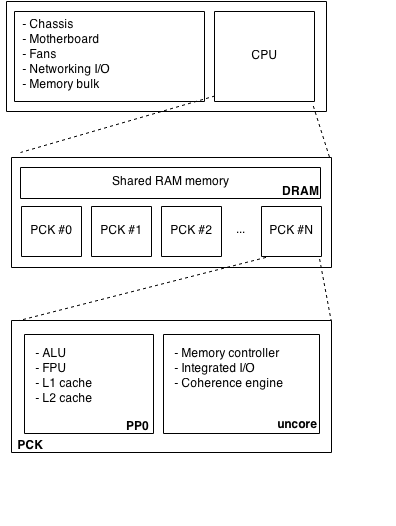
\includegraphics[width=0.5\linewidth]{./figs/energy_system.png}
\vspace{-0.1\linewidth}
\captionsetup{font=scriptsize, width=.75\linewidth}
\captionof{figure}{System's components which contribute for power consumption in HPC}
\vspace{\figurespace}
\end{minipage}

According to our measurements, the power consumption quota of each component varies depending on the system's configuration (see Figure X).  



\section{Techniques and tools overview}
\begin{minipage}[b]{1\linewidth}

\begin{itemize}
\item \textbf{External measurement tools}
It consists of non-invasive clamp meters or electrical plugin power monitors. The external monitoring tools account for energy drained by the whole system or coarse-grained set of components.
\item \textbf{On-chip measurement tools}
It consists of monitoring chips embeeded on the system's SOC to perform fine grained and low resolution measurements.\\
These monitoring chips usually support power measurements on RAM and CPU level (see Figure 1).\\
Intel supports this since its Sandy Bridge models through Running Average Power Limiting (RAPL) technology. Other alternatives, such as the Texas Instrument TI231 power monitor, allow integration of monitoring chips in any architecture. 
\item \textbf{Software Based}
It consists of software applications that predict energy consumed by the system based on energy consumption models. The software can also rely on physical measurements, which increases measurement accuracy\\.
\end{itemize}
\end{minipage}

\section{IgProf}

Software can help to understand how and where energy is consumed in a fine grained scale. For instance, IgProf is a tool for measuring and analysing the applications' memory and performance characteristics.\\ 
IgProf was recently ported to AArch64 and extended with an energy profiling module, which obtains energy measurements from the RAPL interface through the PAPI library. Therefore, it is possible to know how much energy is spent on each function of the application running, which is important for software fine-grained tuning.



% The end of the first column and the start of the second
\end{minipage} % no empty line before the next ``\begin''
\hspace{0.03\linewidth} % Middle margin
\begin{minipage}[t]{0.5\linewidth}
\setlength{\parindent}{10mm} % Paragraph indent

\vspace{\sectionspace}
\section{Energy consumption measurements}


We have performed onchip and external measurements of workloads from CERN running on ARM and Intel architectures. 
The results presented below were obtained by running a typical CERN workload for an average of 30 minutes.
\vspace{\sectionspace}
\subsection*{Machine's specifications}

\begin{description}
  \item[XeonPhi] \hfill \\
  \textbf{CPU}  big, 32 cores. \\
  \textbf{Memory} some teras\\
  \textbf{Notes}  Machine on a rack , ect..
  
  \item[ODROID] \hfill \\
   \textbf{CPU}  not bg, 4 cores. \\
  \textbf{Memory} few gigas\\
\end{description}

\vspace{\figurespace}
\begin{center}
  	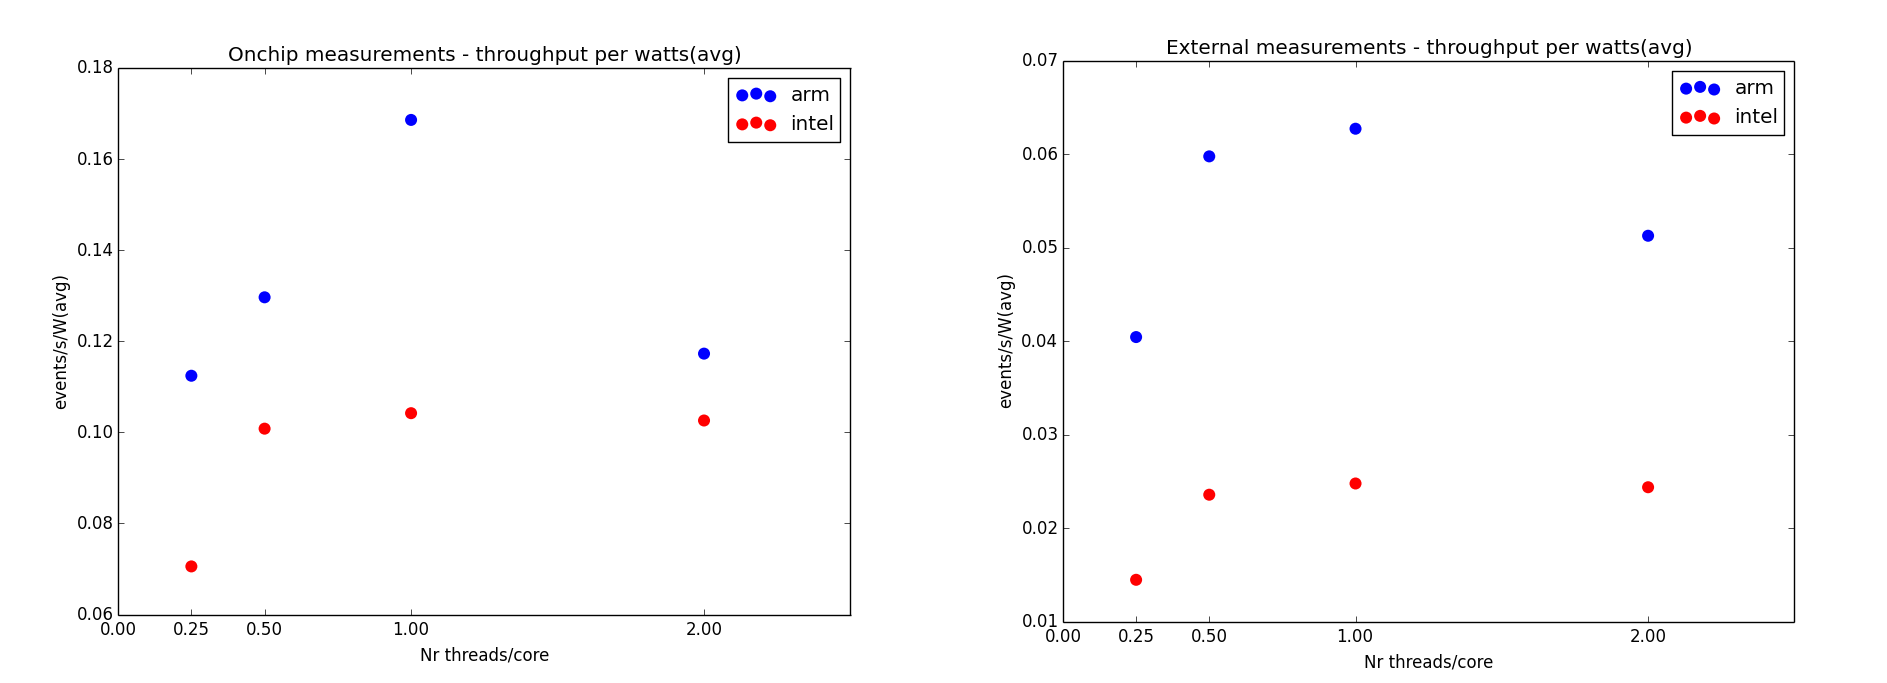
\includegraphics[width=.8\linewidth]{./figs/2measurements.png}
\end{center}
\vspace{\figurespace}


\vspace{0.02\linewidth} 

\subsection{Onchip monitors}
The XeonPhi machine has support to the Intel's RAPL technology. Therefore, it was possible to measure the power consumed on package (PCK), core (PP0) and memory (DRAM) level (see Figure 1).\\
The ODROID machine has a TI INA231 monitoring chip embeeded. This chip allows power monitoring of the CPUs and memory. The results are shown in the Figure 2A.

\vspace{\sectionspace}

\subsection {External physical measurements}
Both XeonPhi and ODROID machines have an external power monitoring tool for measuring the amount of power consumed by the whole system. The results are shown on Figure 2B. In addition, it is possible to see on Figure 3 the ratio between the different components and compare it with the overall energy consumed during the tasks.
\vspace{\figurespace}

\begin{center}
  	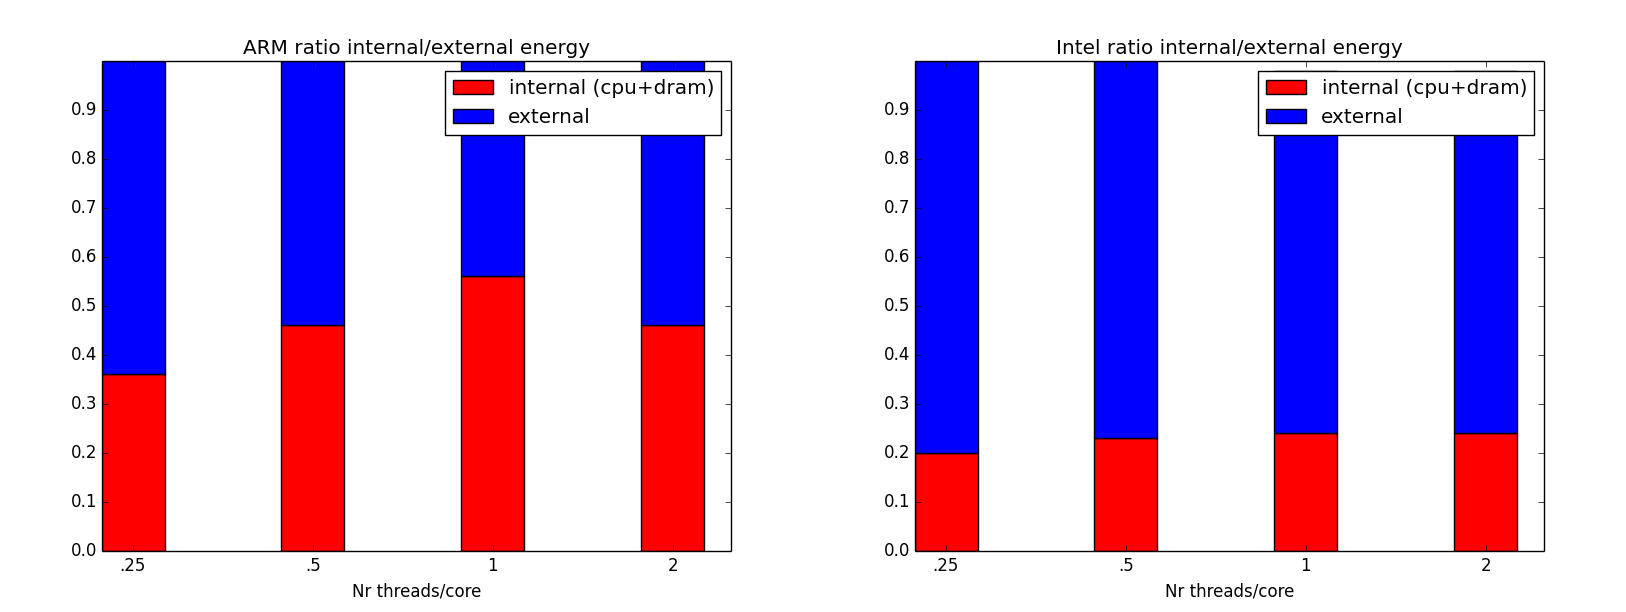
\includegraphics[width=.85\linewidth]{./figs/2ratio.png}
\end{center}
\vspace{\figurespace}


\vspace{\figurespace}

%\fbox{
%\begin{minipage}{0.95\linewidth} 
%\vspace{0.03\linewidth} %space between intro and rest
%\section{Conclusion}
%conclusion.\\
%mention IgProf port\\
%conclusions about  measurements\\
%future work\\
%\end{minipage}
%}


%{\tiny % % Bibliography text size begins...
%{\footnotesize % % Bibliography text size begins...
%\begin{thebibliography}{1}
%\bibitem{Tretyakov1996}
%S.~A. Tretyakov, F.~Mariotte, C.~R. Simovski, T.~G. Kharina, and J.~P. Heliot,
%  ``Analytical antenna model for chiral scatterers: comparison with numerical
%  and experimental data,'' \emph{{IEEE} Trans. Antennas Propag.}, vol.~44,
%  no.~7, pp. 1006--1014, 1996.
%\end{thebibliography}
%} % <- bibliography text size ends


\end{minipage}
\end{minipage} % minipage for the two columns (minipages)





%\vfill % Fill the free space until the footer minipages


%\begin{minipage}{0.95\linewidth} % Minipages for the footers


%\footnotesize % Text size for footers
%\vspace{0pt}
%\textsf{\textbf{Authors and institutions \& Aalto, CERN, FermiLab, others\\
%contacts@..com}}
%\end{minipage} % No empty line before the second begin!
%\hspace{0.03\linewidth}
%\begin{minipage}[t]{0.47\linewidth} % Footer #2
%\vspace{0pt}
%\textsf{\textbf{Authors and institutions \& Aalto, CERN, FermiLab, others\\
%contacts@..com}}
%\end{minipage}
%\end{minipage}


\end{document}
